
\documentclass[12pt]{article} %style

\usepackage[utf8]{inputenc}
\usepackage[T1]{fontenc}
\usepackage{lmodern}
\usepackage[colorlinks=true,urlcolor=black,linkcolor=blue]{hyperref}
\usepackage{graphicx}
\usepackage{wrapfig}
\usepackage{array}

\let\origdoublepage\cleardoublepage
\newcommand{\clearemptydoublepage}{%
	\clearpage
	{\pagestyle{empty}\origdoublepage}%
}

\renewcommand{\arraystretch}{1.2}

\newenvironment{montabular}[1]{\par\vspace{0.3cm} % 4 motifs = {nom} [nombres d'argument] {début} {fin}
\begin{tabular}{#1}}
{\end{tabular}
\vspace{0.3cm}\par}

\makeatletter
\def\clap#1{\hbox to 0pt{\hss #1\hss}}%
\def\ligne#1{%
	\hbox to \hsize{%
	\vbox{\centering #1}}}%
\def\haut#1#2#3{%
	\hbox to \hsize{%
	\rlap{\vtop{\raggedright #1}}%
	\hss
	\clap{\vtop{\centering #2}}%
	\hss
	\llap{\vtop{\raggedleft #3}}}}%
\def\bas#1#2#3{%
	\hbox to \hsize{%
	\rlap{\vbox{\raggedright #1}}%
	\hss
	\clap{\vbox{\centering #2}}%
	\hss
	\llap{\vbox{\raggedleft #3}}}}%
\def\maketitle{%
	\thispagestyle{empty}\vbox to \vsize{%
	\haut{}{\@blurb}{}
	\vfill
	\vspace{1cm}
	\begin{flushleft}
		\usefont{OT1}{ptm}{m}{n}
		\huge \@title
	\end{flushleft}
	\par
	\hrule height 4pt
	\par
	\begin{flushright}
		\usefont{OT1}{phv}{m}{n}
		\Large \@author
		\par
	\end{flushright}
	\vspace{1cm}
	\vfill
	\vfill
	\bas{}{\@location, the \@date}{}
	}%
	\cleardoublepage
}

\def\date#1{\def\@date{#1}}
\def\author#1{\def\@author{#1}}
\def\title#1{\def\@title{#1}}
\def\location#1{\def\@location{#1}}
\def\blurb#1{\def\@blurb{#1}}
\date{\today}
\author{}
\title{}
\location{Amiens}\blurb{}
\makeatother
\title{Second year intern-ship}
\author{Mathilde Andre}
\location{Chamb\'ery}
\blurb{%
		D\'eveloppeur technologie Java J2E / Ajax OS Debian\\
		Host company : Pentila Nero \\
		Jury members : Christophe Rippert and V\'eronique Dudley-Beguin\\
}%
\begin{document}
\maketitle
\renewcommand{\contentsname}{Table of contents}
\tableofcontents
\cleardoublepage

\section*{Introduction}
\addcontentsline{toc}{section}{Introduction}
Introduire le sujet et l’articulation du rapport (2-3 paragraphes)

Within the studies at the Enginiering school ENSIMAG in Grenoble, every student has
to attend a two months internship within a company of his choice.
I worked with the 10 years old company named Pentila, located in Chambéry. 
This internship hold my attention because it was about web development which is a field 
that I wanted to know better. The application that I had to work on used modern
dynamic web technologie. \\  


This company develop a digital workspace inspired from the elcetronic schoolbag, it has
the same goals and functionalities. It aims to facilitate the flow of information between 
teachers, students and parents. \\

During this internship I had many tasks to do for the company that I could split into 3 main
areas that would be the development of my report.  
I will first discribe the company within the context of my work.
Then I will focus of the main tasks I had to do. First, I will explain the softwares 
installations I did for the company, why and how I did them. I will then move on the testing
area and the differents kind of testing I did. Finally I will explain how I fix the bugs 
found during the testing part. The last section would be about my feelings and outcome
learning of this internship.  

\cleardoublepage

\section{Overview and context}

Présenter le contexte dans lequel vous avez effectué votre stage : description de l’entreprise en lien avec le stage : organisation, enjeux pour l’entreprise, qui vous à encadré (une personne, une équipe, ...) (1 page maximum). Le «copier/coller» des sites web des entreprises est à proscrire !

\subsection{The company}

Pentila is a small company with 4 employees. They develop an application which is an electronic schoolbag. 
It is already used in some schools, especialy in Rhone Alpes. 
This application allows the educationnal community to . Parents can know their children's homeworks as well as their schedule. Students can hand in homework to their teachers directly on the website. It makes relation between school, parents and students easier. 

But as in all company, you always have to improve your work. My tasks were mostly to help installing some new software useful for the application or for the team work, but also to find bugs into their application and later fix them.  

They all work on MAC computer and I had a computer with Debian. The OS was fresh installed so it didn't have any work environment for the application. 






\cleardoublepage

\section{Goals}


Présenter les objectifs du stage afin que vos évaluateurs cernent bien la limite entre l’existant et votre contribution réelle : (environ 5 pages)
\begin{itemize}
	\item le travail à réaliser ou le problème à résoudre
	\item l’état de l’art des solutions existantes et des contraintes fixées par l’entreprise
	\item votre solution motivée à partir de l’analyse ci dessus
\end{itemize}


---------------------------------------------------------------

My tasks were related to differents fields such as installing new software for the team of deveopers, finding new bugs and reporting them into an application then fixing bugs. 
That's why I will present these tasks separately. 

\subsection{Instalation of Redmine}
Redmine is a software for project management and bug-tracking. I had to install this application in order to allow the team to track bugs in their app. \\ 
It was very useful for them to have an access into Redmine directly from their IDE (Eclipse). 
Hopefully, Redmine has several useful plugins available so I had to do some researchs to know which one could be useful for the developers, the goal was to make their work faster. Once this research done I had to install the plugins into Redmine. \\ 
The last step was to set up the Redmine's environment to allow the developers to use it easily.


\subsection{Bugs tracking}

\begin{itemize}
	\item Functionality tests
	\item Installation of JMeter
\end{itemize}

\subsection{Bugs fixing}


\cleardoublepage

\section{Softwares installation}

Décrire votre travail (environ 6 pages)
\begin{itemize}
	\item architecture de votre solution (vision haut niveau)
	\item implémentation de votre solution (détail technique) ou de la partie la plus intéressante si la place manque

\end{itemize}

In this part I will discuss the diffenrents softwares I have installed for the company. Firstofall I will focus on the research I have done. Then the details of the installation will be detailed. 
\subsection{Researches}


\cleardoublepage

\section{Software Testing}

	The goal of testing software is to provide informations about the quality of the product. 
	It allows developers to know about potential bugs but it also allows the business 
	to appreciate more the product. The testeur write a document with all the 
	functionalities of the application and give it to the customers.\\  

The company has a quite big application and the developers have some code that they didn't develop
 themself. They need to do a lot of software testing, in order to know about
bugs in their application but also about not convenient functionalities. We distinguish 
two kind of testing issues such as bugs and evolutions. 

This step of software development is essential and is quite
long and boring. But thanks to this part, the customers will have a nice application, 
easy to use and without obvious bugs. 
My task was to do system testing. In order to accomplish it, I did black box testing. 
I didn't know anything about the internal stucture and implementation of the application
and I tested functional parts of the website.

I had do to typical testing such as testing the functionalities on the website. 
But, I also had to test more complicated things such as the coherence between 
teacher, parents and students accounts. For example, in the homework notebook service, 
if a teacher add an homework for a class, all his sudents should see it as well as 
	the sudent's parents. \\



But doing some tests without writing anything about them is not very useful for the future 
of the company. That's why my first task was to test all the services of the application and report all the 
functionalities of every services on a document test. 
I learnt how to write lisable tests documents with functionalities plan and it is not so obvious. \\ 

In this part of the report, I will describe my different tasks in software testing. 
I separate software testing in two sections that represent my work for the company: 
Acceptance testing and Resgression testing. So I will first descibe these two kind of 
testing and explain what I did exactly. 
In the last part I will focus on a software that I used a bit for testing : JMeter.  \\

\newpage
\subsection{Acceptance testing}
I named this section Acceptance testing but I will more talk about how to 
write a technical validation report than testing. \\ 

Individual software modules are combined and tested as a group. All the services can be test
together, as it would be for the customers. 
The purpose of these tests is to "proove" that the application works fine and doesn't have
big bugs. So it consists of verifying functional, performance and reliability requirements. 
In order to do that, the company first needed a document that explain the different 
functionalities of the website. This paper will be very useful for the future users of the 
application.  
My first task was to test all the functionalities of the application and report them all in a technical validation report. This document is a measuring tool
which will be very useful to do regression tests. 
As the application is suposed to work in all web browser that the customers
would be likely to use, I had to test the functionalities on these web
browsers. I finally did some tests on three of them : Firefox, Google chrome and
Internet Explorer. \\ 

The first step was to test the functionalities and write them all in a technical validation
 report. In order to do so, I looked in details every services of the application to 
understand well what they were supposed to do. 
As an example, the website had a school bag service and a pigeonhole service.
In the school bag service you could add some documents, oranize all your papers in
differents folders and so on. Then you could drop off some of them in the pigeonhole of an
other user.
All the services had some tricky functionalitie that I needed to know. Then I could write
the technical report easier. 
   
I will give you a detailed example that I wrote in this report. 
It is about the wysiwyg editor. It is used to create some web document. In this system in 
which the user can view something very 
similar to the end result while the document is being created.  \\ 
b \\
b \\
b \\
b \\
b \\
b \\

\newpage
\begin{itemize}
	\item Access to the service\\

\begin{tabular}{|m{4cm}|m{3cm}|m{4cm}|m{2.1cm}|}
\hline
\textbf{Name of the stage} & \textbf{Description}
 & \textbf{Expected result} & \textbf{Comments} \\
\hline
Select Schoolbag service then the Create menu -> Document & 
Opening of the editor Wysiwyg & 
\begin{minipage}{0.7\textwidth}
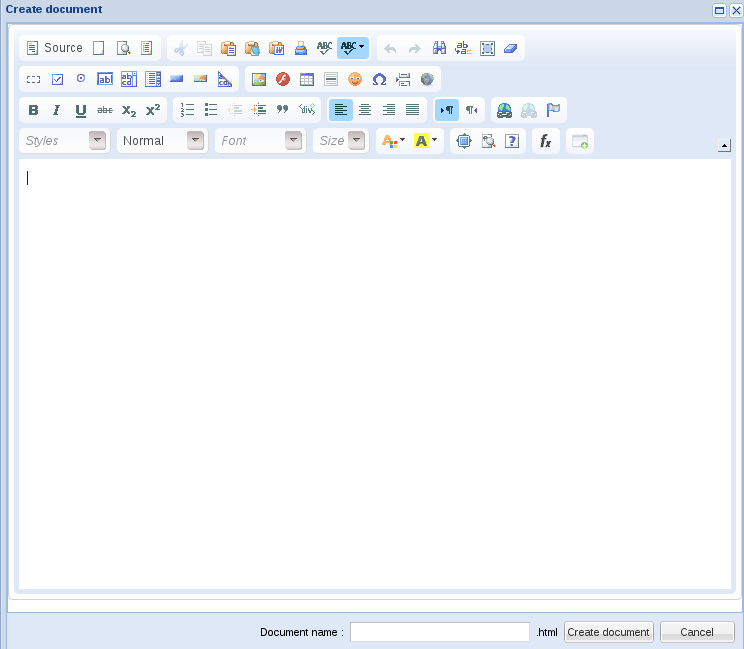
\includegraphics[scale=0.15]{Images/wysi.png} 
\end{minipage}& 
\\
\hline
\end{tabular}
\\
	\item Create a document \\

\begin{tabular}{|m{4cm}|m{3cm}|m{4cm}|m{2.1cm}|}
\hline
\textbf{Name of the stage} & \textbf{Description}
 & \textbf{Expected result} & \textbf{Comments} \\
\hline
\begin{enumerate}
	\item Fill a description of a document

	\item Choose a name : test

	\item Select create document 
\end{enumerate}&
Display of the new document in the list : test.html & 
\begin{minipage}{0.7\textwidth}
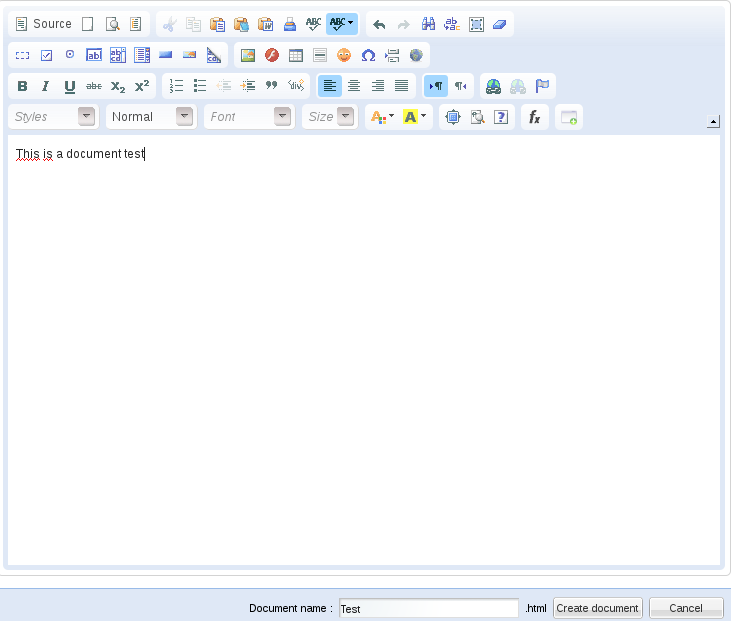
\includegraphics[scale=0.15]{Images/document.png} 
\end{minipage}& 
\\
\hline
\end{tabular}
\\
\end{itemize}

In the report I created one section for each service. Then I accompanied 
each functionality with a formal description of the actions to perform, 
the eventual input data and their expected output. In the comments column, I wrote when the
functionality didn't work well or had a strange beahaviour accoding to me. But then, 
if the comments was some kind of bugs or evolutions, I used Redmine to report them.  
My descriptions has to be as high level as possible in order to be understable for the customers. 

As a result of my work, the company had a useful document. It is now used to do regression
testing as I will explain in the next part. And it could be used to do automated tests later,
 all the scenario to test are already written. And of course it would be given to the customers.
It is quite easy to evaluate the quality of the document, it has to be easy to read for
the regression tests that will consist in following all the steps detailed into it.\\


\newpage
\subsection{Regression testing}
It is a kind of software testing that consists to uncover new softwares bugs
or regression. These tests are done after each changes such as bugs fixing or new
 configurations settings made in the production instance. 
 Indeed, we can manage to fix a bug but 
meanwhile a new bug can appear. So regression testing aim to discover these
kind of new bugs, it helps to determine whether a change in one part of the
 software affects other parts of the software. 
 
 The tests I have done are called black box testing because I didn't know anything yet about
 the interior workings of the application, about the source code. The main advandage of this 
 testing method is that it clearly separates user's perspective from the developer's
 perspective. My role was to be similar to the future users.\\



The following is an example of test I had to do, which one lead to a bug I have found : 
On the school bag service when we clicked on the new Folder button, then on the close button. 
Then we couldn't click again on the new Folder button. The button was still displayed but when we clicked on it nothing would happen. \\

Each time the team published changement in the production instance, I had to do some
regression testing. In order to do these tests, I used the technical report that I wrote
before. I run set of test-cases by folowing the steps discribed in the document. 
For each test, I compare the results obtained with the expected results. 
If there is a correct match for the test, no new bugs had appeared for this functionality.
 If not, I report the bug. \\
 
 To report anything I notice about a step, I used Redmine and created an issue.
 In case of a correct match it can happen that the functionality tested is less convenient
 for the users than before. In this case I had to create an other kind of issue in Redmine,
such as evolution issue. These issues are usually less urgent to do. 
In each issues (bugs and evolutions), I described with precision what I detected. 
It is very  important to know in which environment the bug had been found such as 
windows or debian, Firefox, Google chrome or Internet Explorer as well as 
all the stages needed to reproduce the bug.  \\ 

\newpage
Here is an example of a creation of Redmine issue : \\ 

\fbox{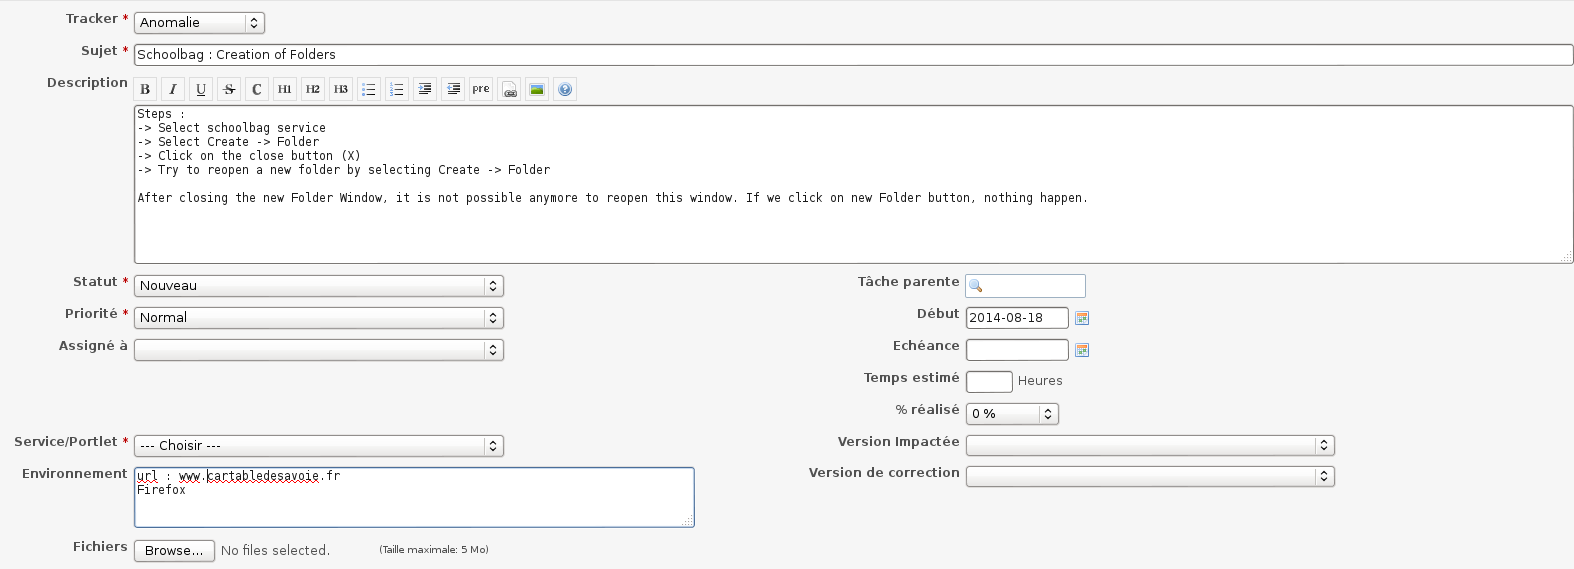
\includegraphics[scale=0.25]{Images/issue.png}} \\

All the redmine issues was then assigned to one member of the team developers and fix by
him. I will talk about this in the part called Bugfix. 


\newpage



\section{JMeter}
		I had to choose an application who fitted the needs of our company : 
		a load testing application open source for measuring the performance of its website.

\subsection{Research}
After doing some research, only two applications held my attention : Jmeter and Gatling.


I have chosen Jmeter even though it was difficult to choose. 
Indeeed, I have read both good and bad commentary on the net. 
Jmeter is older than Gatling, hence we can find more tutorial on the  net. 
Moreover, I have read that it is easier to make graphics results on Jmeter, and I was asked to do some graphics analysis.

\begin{figure}[h]
		
\includegraphics[scale=0.5]{Images/JMeter.jpeg} 
		Apache JMeter is a  pure Java application  that can be used as a load testing tool for analyzing
 and measuring the performance of a variety of services. It was originally designed for testing 
 Web Applications but has since expanded to other test functions. 
\end{figure}
	
\subsection{Implementation}
Installing jmetter was not very complex. I just downloaded the release and verified that my 
environment met the requirements (as java 6 or some optional jars (for jdbc, jms..)).
Then it was possible to run the application.\\

I needed to prepare some scenarios. 
Here is an exemple of scenario I registered : 
\begin{enumerate}
	\item click on this link
	\item create a file
	\item and so on.
\end{enumerate}
I wrote a document with some scenario to execute.\\

In order to register scenario, I needed to first configure the browser to use the jmetter
proxy and then I recorded some script tests into jmeter. 
On Jmeter, we need a Test Script Recorder, in order to record every step of our scenario we do on the website.

We also need to add a Thred Group inside the Test Plan, where the scenario will be recorded thanks to the Recording Controller.
And also an HTTP Request Defaults that we configured : set the web server and the port.
Finally, we can start recording.

\subsection{Results}

Once the scenario is recorded, we start to test with the Thread Group.
The following graphism is an example of what we can have after starting the test. 
The scenario consist in creation of files. We can see all the steps in the tree on the left
part. And we can configure some parameters in the right part.\\ 

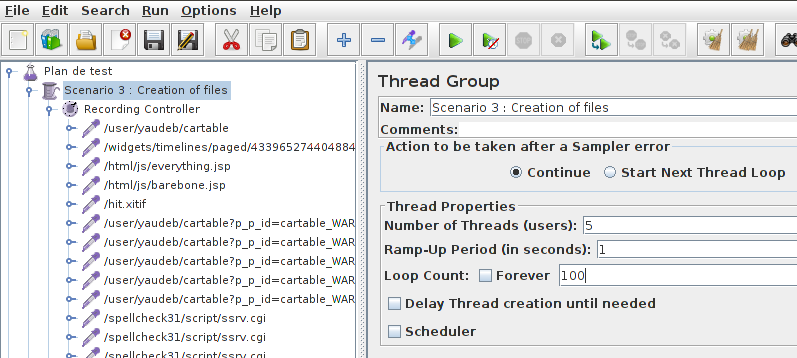
\includegraphics[scale=0.5]{Images/jmetter1.png} 
\\

We set the number of Threads (ex:5) and Loop count (ex:100).
As we can see inside the Recording Controller, a lot of different steps have been recorded. The thred will execute all of them as many times as it is asked to.

We create a summary report to see the results of the execution.

As we can see, it displays every error in each step,  the throughput and so on.

We can also execute some tests with differents users. We write in a file.csv the login and password of some users and add in the application a CSV Data Set Config where we can enter the variables names:LOGIN and MDP (password)  for example.

Then we add the variables inside step of the test. We can see in the tab, near username and password we enter the variables.


It is possible to view some graphics result on Jmeter: \\ 

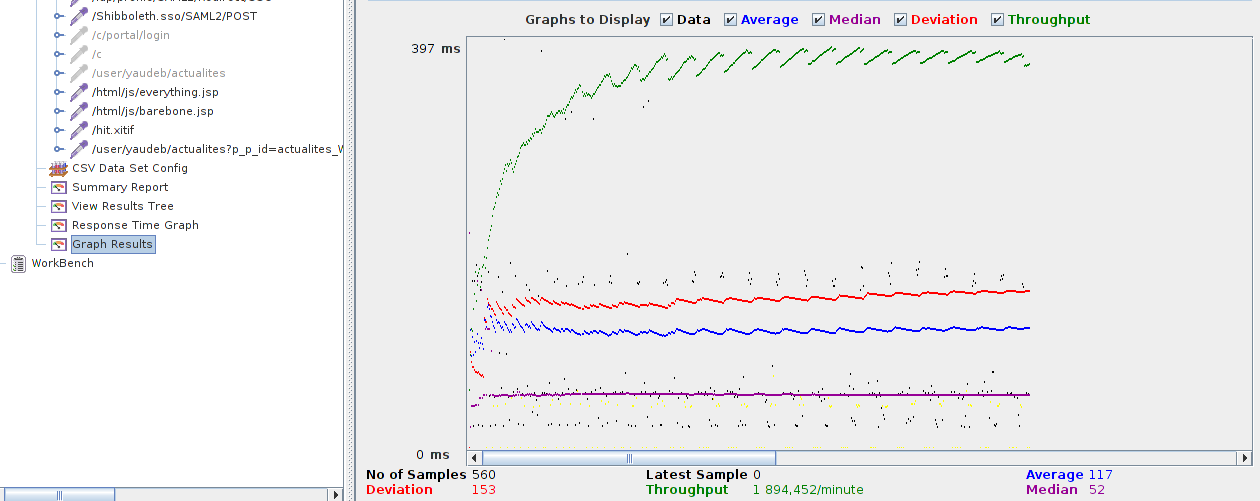
\includegraphics[scale=0.3]{Images/jmetter2.png} 





\cleardoublepage


\section{Bugfix}


\hypertarget{ancre} Expliquer les résultats obtenus et analyser leur cohérence (environ 2 pages)
\begin{itemize}
	\item plateforme de test mise en place, quelles métriques pour évaluer l’efficacité de votre solution
	\item l'adéquation avec les attentes de l’entreprise
	\item les perspectives ouvertes

\end{itemize}


\cleardoublepage

\section{Conclusion}


Faire un bilan personnel du stage : (1 page)
Présenter les obstacles, points durs les plus importants et les moyens entrepris pour les
résoudre ; les compétences interpersonnelles acquises en entreprise
 
  
   
Conclure en résumant ce qui a été effectué durant le stage (2-3 paragraphes)
    




\cleardoublepage

\section{Bibliographic reference}

Références bibliographiques le cas échéant ; une documentation technique déjà rédigée pourra être jointe en annexe.





\cleardoublepage
\end{document}
